\documentclass[11pt]{article}
    \title{\textbf{Tetrahedral mesh orthogonality optimization for solving diffusive problem with finite volume solver}}
    \author{Moie Rousseau}
    \date{}
    
    \addtolength{\topmargin}{-3cm}
    \addtolength{\textheight}{3cm}
    
\usepackage{amsmath}
\usepackage{graphicx}


\begin{document}

\maketitle
\thispagestyle{empty}

\section*{Abstract}

TODO

\section{Introduction}

Numerical simulation. 
Discretization method. 
Finite volume solver. 
Discretization of diffusion operator.
TPFA vs MPFA. Advantage of TPFA. PEBI grid.
Several software use the TFPA for the diffusion operator, for example PFLOTRAN \cite{hammond_pflotran_2012}, DuMux \cite{koch_dumux_2021}, PorePy \cite{keilegavlen_porepy_2021}, Open Porous Media flow simulation \cite{rasmussen_the_2021} or OpenFOAM \cite{}, Waiwera %https://waiwera.readthedocs.io/en/latest/setup_mesh.html
Require orthogonal mesh.

However, orthogonal meshes are rather the exception than the rule, and non-orthogonal meshes could introduce a $O(1)$ error which cannot be reduced by refining the mesh elements.
Cartesian meshes.
Octree meshes.
Voronoi meshes: often not conformal and relying on clipping to fit the modeled domain.
Recent research provide quasi-conformal Voronoi meshes by minimizing the volume of cells empassing a 2D feature \cite{merland_voronoi_2014} or by placing seeds such as no clipping is required \cite{abdelkader_vorocrust_2020}.
Also, there is many mesher available for generating tetrahedral meshes such as gmsh \cite{geuzaine_gmsh_2007}, TetGen \cite{si_tetgen_2015}, NETGEN \cite{schoberl_netgen_1997}, CGAL \cite{}, or Vorpalite \cite{} among others.

Non-orthogonal meshes such as tetrahedral can still be used along with a appropriated correction such as the deferred correction approach \cite{jasak_error_1996, moukalled_finite_2016}.
Describe it.
However, the more the mesh is non-orthogonal, the more iteration it will takes + error \cite{traore_robust_2009}. %it's a guess here, so I need to find reference
Therefore, improving mesh orthogonality is a way to enhance accuracy of the numerical solution and decrease computational time.

Variational approach to mesh orthogonality

This study presents an approach for optimizing the tetrahedral mesh orthogonality in order to reduce numerical simulation error and computational time.
Approach is decribed and tested for several mesh and diffusive problem.
Calculation made with OpenFOAM.

Mesh orthogonality: normal scalar cell center vector superior to 1/3 is good %file:///tmp/mozilla_moise0/MeshQuality-Appendix-A.pdf
openfoam: angle of non orthogonality > 5° require the correction, slow convergence for mesh orthogonality above 80° %https://www.sciencedirect.com/science/article/pii/S0029549317300596 (see for cell center)

They look for orthogonality: 
%https://www.sciencedirect.com/science/article/pii/S0360544215009068?casa_token=2XncBO8cC2EAAAAA:2ElyHYXlp_7U6AfgEwTn-F8ZWls7tZbjbetgQ6Cm00bxm20JBejOxlf4Go2EnBZUhaajeYneAQ#bib22
%https://pdfs.semanticscholar.org/1d52/a4f30ed56bb82791c283eba37d15eee582cd.pdf
%https://sci-hub.wf/10.1051/e3sconf/20171401027




\section{Mesh optimization}


\subsection{Formulation of optimization problem}

Boundary faces did not needed to be optimized (it lack a point to define the cell center vector).
Cell of a prisms not considered. Tet and pyramid are optimized. Cell must be either hexa, pyr or tet.

The objective of the optimization was to minimize, for each face, the angle between the face normal and the vector connecting the two cells center sharing the considered face by moving the mesh vertices. 
Therefore, the objective function to minimize was defined as follow:
%
\begin{equation}
\begin{aligned}
& \underset{P}{\text{minimize}}
& & c(P) = \sum_{f \in faces} E_f \left( r_f^T \cdot n_f, w_f \right)  \\
& \text{subject to}
& & r_f^T \cdot n_f \geq 0, \\
& & & P = \{P_i  \} \\
\end{aligned}
\label{eq:opt_problem}
\end{equation}
$E_f$ is the individual face error defined as a function of the $r_f$ the unit vector in the direction connecting the two cell center sharing the considering face $f$ and $n_f$ the unit face normal (Figure).
The optimization variables $P$ represent the set of mesh points $P_i$ not lying on the boundary %TODO. 
%The dot product give the cosinus of the face normal - cell center vector angle which is maximal when both vector are aligned (i.e. the mesh orthogonal at this face). 
The $w_f$ is a user specified weighting constant factor which allowed give higher importance to some connections compared to other.

Choosing the right function $E_f$ is critical to ensure both a effective mesh orthogonality optimization and the creation of non-inverted elements. 

Minimizing $c$ therefore contributes to decrease the overall non-orthogonality error of the mesh.
This optimization problem constitute a high dimensional problem, while 3D tetrahedral meshes nowaday contains at several thousands of points, and up to billion sometimes \cite{neau_massively_2020}.
Therefore, optimization was carried out using a gradient descent method such a the BiCGStab algorithm \cite{}.
This method requires the derivative of the objective function relative to all the point in the mesh, which is detailed in the following section.

%TODO say we are optimizing point belonging to triangle, not quad, because of an additional equality constraint


\begin{figure}[h]
  \centering
  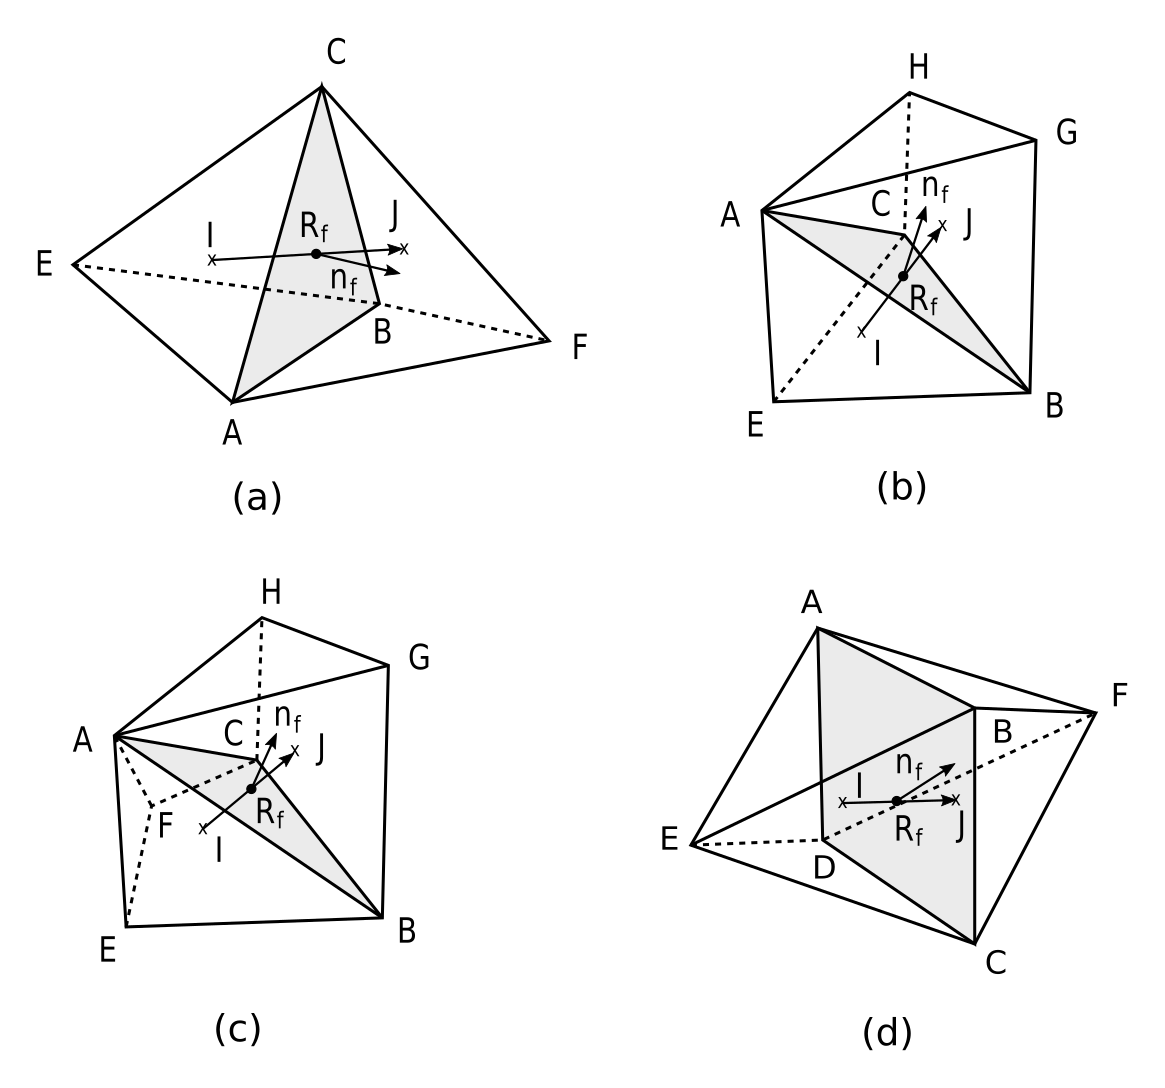
\includegraphics[width=0.9\textwidth]{figures/cases.png}
  \label{cases_figure}
  \caption{Example configuration}
\end{figure}


\subsection{Derivation of the objective function}

\subsubsection{General expression}

Using gradient base algorithm to solve the optimization problem (\ref{eq:opt_problem}) require the knowlegde of the objective function derivative relative to each point $P_i$ of coordinates $(x_i,y_i,z_i)$, which can expressed as the sum of the derivative of each individual face error $d E_f / dP_i$:
%
\begin{equation}
\frac{dc}{dP_i} = \sum_{f \in faces} \frac{d E_f}{d P_i}
\end{equation}
%
However, for a given mesh face $f$, if the two elements sharing the face $f$ do not contains the mesh point $P_i$, the derivative ${d E_f}{d P_i}$ will be null.
In fact, there is only few cases when the derivative is non-null, which can be grouped into three configurations (Figure X):
\begin{itemize}
\item the considered point is a face point (configuration $P_i = A$),
\item the considered point belong to the element pointed by the face normal (configuration $P_i = F$),
\item or the belong to the other element (configuration $P_i = E$).
\end{itemize}
%
The derivative of individual face error $E_f$ according to a mesh vertices $P$ could be therefore be simplified to read:
%
\begin{equation}
\frac{dE_f}{dP} = \sum_{f\in\ conf(P=A)} \frac{dE_f}{dA} + \sum_{f\in\ conf(P=E)} \frac{dE_f}{dE} +
\sum_{f\in\ conf(P=F)} \frac{dE_f}{dF} 
\end{equation}
%
where $f \in conf(P=X)$ states for the faces $f$ for which the point $P$ is in configuration $X$ (either ($A$, $E$ or $F$). 


\subsubsection{Individual face error derivative}

The general formula of the derivative of individual face error $E_f$ according to a mesh vertice $P_i$ is given by:
%
\begin{equation}
\frac{dE_f}{dP_i} = E'_f\left( r_f^T \cdot n_f, w_f \right) \left(n_f^T \cdot \frac{d r_f}{dP_i}\ +\ r_f^T \cdot \frac{d n_f}{dP_i}\right)
\label{general_derivative_expression}
\end{equation}
%
Where $E'_f$ is the weighting function derivative relative to its face orthogonality variable $(r_f^T \cdot n_f)$.
The evaluation of individual face error derivative (equation \ref{general_derivative_expression}) required the derivative of the face normal vector relative to the considered point $d n_f / dP_i$ and those of the cell center vector $d r_f / dP_i$, which are unit vector whose coordinates does not depend trivially on the mesh point $P_i$.
Expanding the unit vector derivative $du/dP_i$ to link it with its dimensional counterpart leads $dU/dP_i$ (see Annex A):
%
\begin{equation}
\frac{du}{dP_i} = \frac{1}{N} \left[ \boldsymbol{I} - \frac{1}{N^2}\ U \otimes U^T \right] \frac{dU}{dP_i}
\end{equation}
%
The previous formula could therefore be used to calculate the derivative of unit vector $n_f$ and $r_f$ relative to any mesh point $P_i$.

\subsubsection{Unit normal derivative}

The dimensional face normal $N_f$ of a triangle face $ABC$ (other face are considered fixed) could be computed using the cross product of two of its edges, for example $AB$ and $BC$.
Chosing $A = P_i$, and derivating the cross product relative to $A$ leads:
%
\begin{equation}
\frac{d N_f}{dA} = \frac{d (B-A) \times (C-B)}{dA} = \begin{pmatrix}
0 & (b_z-c_z) & (c_y-b_y) \\
(c_z-b_z) & 0 & (b_x-c_x) \\
(b_y-c_y) & (c_x-b_x) & 0
\end{pmatrix} 
\end{equation}
%
Where $B$ and $C$ are the two others triangle points taken in arbitrary order.
Therefore, the term in equation (\ref{general_derivative_expression}) implying the derivative of the unit normal $n_f$ is given by, after rearranging parentesis near the dyadic product product:
\begin{equation}
r_f^T\cdot \frac{d n_f}{dA}\ = 
 \frac{1}{\| N_f \|} \left[ r_f^T -  (r_f^T \cdot n_f)\ n_f^T \right] \frac{d N_f}{dA}
 \label{deriv_n_f}
\end{equation}
%
Which can be more compactly writed as:
%
\begin{equation}
r_f^T\cdot \frac{d n_f}{dA}\ = 
 \frac{1}{\| N_f \|} \left[ \left[ r_f^T -  (r_f^T \cdot n_f)\ n_f^T \right]^T \times (C-B) \right]^T
\end{equation}



\subsubsection{Unit cell center derivative}

General expression of the (dimensional) cell center vector $R_f$ writes:
\begin{equation}
R_f = J-I
\end{equation}
with $J$ the center of the element pointed by the face normal direction and $J$ in the opposite direction.
Element (mass) center as a function of the element vertices are given in Table \ref{}.

\begin{table}
\begin{tabular}{|l|l|}
\hline
	Element type & Element center $X$\\ \hline
	Tetrahedron (ABC-E) & $X = (A+B+C+E)/4$\\ \hline
	Pyramid (ABCD-E) & $X = $\\
	Wedge (ABC-EFG) & 42\\
	51 & 52\\
\hline
\end{tabular}
\end{table}


Cell center vector depend of the two element types shared by the given face.
In this study, four elements types 

Derivative of cell center vector and face normal according to mesh vertices required the knowledge of of the configuration of the mesh near the considered faces. Four distinct cases were identified (see X):
\begin{enumerate}
  \item Face is a triangle shared by two tetrahedra (common case). 
  \item Face is a triangle shared by one tetrahedron and one pyramid.
  \item Face is a triangle shared by two pyramids.
  \item Face is a quad shared by two pyramids
\end{enumerate}

In each case, the problem was generalized as follow: let $A$, $B$, $C$ (and $D$) be the three (four) vertices of the considered triangular (quad) face. 
Let $I$ and $J$ be the center of the two cells sharing the considered face so that the vector $R_f=\|R_f\|\ r_f = \overrightarrow{IJ}$ and the face normal $n_f = \overrightarrow{AB} \cdot \overrightarrow{AC}$ point in the same direction (i.e. $r_f^T \cdot n_f \geq 0$).
Vertices $E$ and $F$ designed the last vertices of the tetrahedra (pyramid) of center $I$ and $J$ respectively (see X).
The general problem was therefore to find the derivative of face area $ABC(D)$, the normal vector $n_f$ and the cell center vector $r_f$ according to mesh vertice $P$ if $P$ is either $A$, $E$ or $F$ ($B$, $C$ and $D$ cases are recovered by simply reordering face vertices). 



\subsection{Numerical implementation}

A example implementation is proposed (REF) and uses the C++ programming language. 
This program takes as input the vertices coordinate in xyz format, the mesh element topology and the optimization parameters. 
Then, the mesh is decomposed and the internal connections are built. Optimization is carried using a on-purpose class call OrthOpt which compute the objective function and the derivative according to vertice position. 
Finally, optimization is carried using the L-BFGS algorithm of the L-BGFSpp library (REF). Stopping criteria include the maximum number of iteration, ..

The proposed implementation also benefits from the parallelization using OpenMP up to an arbitrary number of threads. 

Speed up.



\section{Application to numerical simulation}

\subsection{Example problem}

The equation solved. The problem. The mesh.

Solve with OpenFOAM.

Must have a analytic solution. 
%example: https://www.openfoam.com/documentation/tutorial-guide/2-incompressible-flow/2.2-flow-around-a-cylinder#x7-390002.2

\subsection{Orthogonality optimization}

Use different penalization power, initial weighting factor. 
For example, considered $n=1$, $n=3$ and $n=0.5$.

Plot before / after.

\subsection{Numerical simulation results}

Simulation with original mesh without correction, with correction.

Compare accuracy to optimized mesh using the different penalization power.

Compare simulation time.

\section{Results analysis}

\subsection{Penalizing high error}
High orthogonality error could be more penalized by applying a power-law to individual face error. 

One may want to weigth the cost function with the face area in order to avor face orthogonality with high area. 
This weighting had also the advantage of possessing a less complicate derivative. 
However, meshes are often refined in sensitive place with low area faces, and therefore, this weigthing could be counter-productive in that case.

\subsection{Discussion}

Anisotropy can't work.
Unless grid are K orthogonal \cite{heinemann_modelling_1991}.
However, no possible for tetrahedron

Conventional two-point flux approximation (TPFA) can only obtain the flux normal to the grid interface but completely neglects the one parallel to it \cite{}. MPFA needed. %https://ui.adsabs.harvard.edu/abs/2017AGUFM.H31D1541L/abstract

Inverted element.

Further work.
2D case.
Weighting factor as a function of the configuration.
Include skewness error for gradient operator


\section{Conclusion}

TODO



\bibliography{references.bib}
\bibliographystyle{apalike}


\clearpage


\section*{Annex: Derivative of the objective function}

\subsection*{A. Unit vector derivative relative to a point}
Starting from the definition of a unit vector $u$:
\begin{equation}
u = \frac{U}{N}
\end{equation}
With $U$ a non unit vector and $N$ its norm.
Derivate according to a particular point $X$ write:
\begin{equation}
\frac{du}{dX} = \frac{1}{N^2} \left[ N \frac{dU}{dX} - U \otimes \frac{dN}{dX} \right]
\end{equation}
Where the sign $\otimes$ represent the dyadic product. Derivative of the vector norm $N$ expresses:
\begin{equation}
\frac{dN}{dX} = \frac{d}{dX} \sqrt{\sum_i U_i^2} =
\frac{1}{N} \sum_i U_i \frac{dU_i}{dX}
\end{equation}
Which simplifies to:
\begin{equation}
\frac{dN}{dX} = \frac{1}{N}\ U^T \frac{dU}{dX}
\end{equation}
Replacing the above expression in those of the derivative of the unit vector $u$ leads, after dyatic product rearangement and factorization:
\begin{equation}
\frac{du}{dX} = \frac{1}{N} \left[ \boldsymbol{I} - u \otimes u^T \right] \frac{dU}{dX} = \frac{1}{N} \left[ \boldsymbol{I} - \frac{1}{N^2}\ U \otimes U^T \right] \frac{dU}{dX}
\end{equation}
With $\boldsymbol{I}$ the unit 3x3 diagonal matrix.


\subsection*{B. Expressions of cell center vectors and their derivative}

\subsubsection*{Case 1}

Center of a tetrahedra is given by the arithmetic mean of its four vertices:
\begin{subequations}
\begin{gather}
I = \frac{1}{4} (A + B + C + E) \\
J = \frac{1}{4} (A + B + C + F)
\end{gather}
\end{subequations} 
Therefore, cell center vector $R_f$ reads:
\begin{equation}
R_f = \| r_f \|\ r_f = J-I = \frac{1}{4} (F - E)
\end{equation}
Which permitted to express the derivative of $R_f$ according to a mesh vertice $P$ depending if $P$ is either $A$, $E$ or $F$:
\begin{subequations}
\begin{align}
\frac{d R_f}{d A} &= \ 0 \\
\frac{d R_f}{d F} &= - \frac{d R_f}{d E} = \frac{1}{4}\ \boldsymbol{I}
\end{align}
\end{subequations} 

\subsubsection*{Case 2}

In the second case, the center of the tetrahedra $I$ and of the pyramid $J$ are given by:
\begin{subequations}
\begin{gather}
I = \frac{1}{4} (A + B + C + E) \\
J = \frac{A}{4} + \frac{1}{16} (B + C + G + H)
\end{gather}
\end{subequations} 
Therefore, cell center vector $R_f$ reads:
\begin{equation}
R_f = J-I = -\frac{E}{4} - \frac{3}{16} (B + C) + \frac{1}{16} ( G + H)
\end{equation}
In this case, only the $A$ and $E$ point are non fixed. Derivative of the cell center vector according to these two points is thus:
\begin{subequations}
\begin{align}
\frac{d R_f}{d A} &= \ 0 \\
\frac{d R_f}{d E} &= - \frac{1}{4}\ \boldsymbol{I}
\end{align}
\end{subequations}


\subsubsection*{Case 3}

Center of both pyramids are given by:
\begin{subequations}
\begin{gather}
I = \frac{A}{4} + \frac{1}{16} (B + C + K + L) \\
J = \frac{A}{4} + \frac{1}{16} (B + C + G + H)
\end{gather}
\end{subequations} 
Cell center vector $R_f$ reads:
\begin{equation}
R_f = \frac{1}{16} ( G + H - K - L)
\end{equation}
In this case, only point $A$ is non fixed, which therefore give:
\begin{equation}
\frac{d R_f}{d A} = \ 0 
\end{equation}


\subsubsection*{Case 4}

Center of both pyramids are given by:
\begin{subequations}
\begin{gather}
I = \frac{E}{4} + \frac{1}{16} (A + B + C + D) \\
J = \frac{F}{4} + \frac{1}{16} (A + B + C + D)
\end{gather}
\end{subequations} 
Cell center vector $R_f$ reads:
\begin{equation}
R_f = \frac{1}{4} (F-E)
\end{equation}
And derivative is:
\begin{equation}
\frac{d R_f}{d F} = - \frac{d R_f}{d E} = \frac{1}{4}\ \boldsymbol{I}
\end{equation}



\subsection*{C. Expressions of the derivatives}

\subsubsection*{Unit cell center vector term}

Derivative of the unit cell center vector $r_f$ according to a point $P$ write (see Annex A):
\begin{equation}
\frac{d r_f}{dP}\ = 
- \frac{1}{\| R_f \|} \left[ \boldsymbol{I} - r_f \otimes r_f^T \right] \frac{d R_f}{dP}
\end{equation}
Also, the cell center vector derivative is either 0 for $P$ in position $A$, $\boldsymbol{I} /4$ if $P$ is in position $F$ or the opposite if in position $E$ (if non fixed, see Annex B). 
Therefore, the term implying the unit cell center vector in Eq. (\ref{general_derivative_expression}) write:
\begin{equation}
n_f^T\ \frac{d r_f}{dF}\ = - n_f^T\ \frac{d r_f}{dE} =
 \frac{1}{4 \| R_f \|} \left[n_f^T- n_f^T \cdot (r_f \otimes r_f^T) \right]
\end{equation}
Rearranging the parentesis finally lead to the general expression of the unit cell center vector derivative:
\begin{subequations}
\begin{align}
n_f^T\ \frac{d r_f}{dA}\ &=  0 \\
n_f^T\ \frac{d r_f}{dE}\ &= - \frac{1}{4 \| R_f \|} \left[ n_f^T - (n_f^T \cdot r_f)\ r_f^T \right] \\
n_f^T\ \frac{d r_f}{dF}\ &=  \frac{1}{4 \| R_f \|} \left[ n_f^T - (n_f^T \cdot r_f)\  r_f^T \right]
\end{align}
\end{subequations} 



\end{document}